\documentclass[12pt, a4paper, oneside, openright]{book}
\pdfpagewidth\paperwidth
\pdfpageheight\paperheight
\usepackage{graphicx}
\usepackage{subfigure}
\usepackage{hyperref}
\usepackage{amsmath}
\usepackage{amsthm}
\usepackage{amsfonts}
\usepackage{amssymb}
\frenchspacing
\makeatletter
\let\@orig@endthebibliography\endthebibliography 
\renewcommand\endthebibliography{% 
  \xdef\@kept@last@number{\the\c@enumiv}% 
  \@orig@endthebibliography} 

\newenvironment{thesitography}[1] 
  {\def\bibname{Sitografia}% 
   \thebibliography{#1}% 
   \setcounter{enumiv}{\@kept@last@number}% 
} 
  {\@orig@endthebibliography} 
\makeatother
\begin{document}
\pagestyle{myheadings}
\begin{titlepage}
\begin{center}
{{\Large{\textsc{Universit\`{a} degli studi di Firenze}}}} \rule[0.1cm]{15.8cm}{0.1mm}
\rule[0.5cm]{15.8cm}{0.6mm}
{\small{\bf SCUOLA DI INGEGNERIA\\
Corso di Laurea Magistrale in Ingegneria Informatica}}
\end{center}
\vspace{15mm}
\begin{center}
{\LARGE{\bf Testing of chosen Design Patterns}}\\
\vspace{3mm}
{\LARGE{\bf with JUnit and Mockito}}\\
\end{center}
\begin{figure}
\centering

\includegraphics[scale=0.2]{./LaTeX_extra/logo-unifi-1.png}
\end{figure}
\vspace{32mm}
\par
\noindent
\begin{minipage}[t]{0.55\textwidth}
{\large{\bf Docente\\
Prof. Enrico Vicario}} \\
\end{minipage}
\hfill
\begin{minipage}[t]{0.47\textwidth}\raggedleft
{\large{\bf Relazione a cura di\\
Niccolo' Fabbri\\
Francesco Santoni}}
\end{minipage}
\vspace{12mm}
\vspace{12mm}
\begin{center}
{\large{\bf Firenze,\\%inserire il numero della sessione in cui ci si laurea
24 Agosto 2016 }}%inserire l'anno accademico a cui si è iscritti
\end{center}
\end{titlepage}

\mainmatter
\pagenumbering{roman}
\newpage\null\thispagestyle{empty}
\null\vspace{\stretch{0.6}}
\pagenumbering{gobble}
\frontmatter
\clearpage
\tableofcontents
\cleardoublepage
\mainmatter

\chapter{Introduction}
\markboth{Introduction}{\textit{Introduction}}

77777777777 VUOTO PER ORA

\chapter{Design Patterns}
\markboth{Design Patterns}{\textit{Design Patterns}}
In software engineering, a software design pattern is a general reusable template to solve a commonly occurring problem within a given context.

We will study:
\begin{enumerate}
	\item Structural patterns: Adapter(both in his Class and Object variants), Proxy, Decorator, Composite.
	\item Behavioural patterns: Observer, State, Visitor.
\end{enumerate}


\section{Class Adapter}
 Adapts a pre-existent class to a new interface through inheritance. 
 
 Through the new interface the old methods can be directly presented, modified, produce aggregated results or completely new functionality can be added. 
 
 
\subsubsection{Class Diagram}
\begin{figure}[!h]
	\centering
	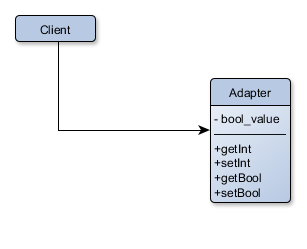
\includegraphics[width=0.3\textwidth]{./Adapter/Class/ClassDiagram.png}
	\caption{Class Adapter: Class Diagram }
	\label{CAclassDiag}
\end{figure}

\begin{itemize}
	\item \textbf{Adaptee}: legacy class with specific methods and fields
	\item \textbf{Target}: desired interface
	\item \textbf{ClassAdapter}: inheriting from Adaptee and Target both, adapts the legacy methods to the desired interface  
\end{itemize}

\subsubsection{Fault Model}
Given that the pattern focuses on allowing access to legacy methods through a new interface, failures are found in the following situations:  
\begin{itemize}
	\item the adapter did not inherit from the legacy class or the new interface
	\item the adapter for some reason cannot interact with the legacy methods 
\end{itemize}

\subsection{Testing}
To negate the two source of failures we reasoned that it is sufficient to test the ways in which the variable \textit{bool\_value} interacts with the methods:

\begin{itemize}
	\item having represented the field's interaction with the class methods through a data flow graph whose basic blocks are methods, we decided to test them following the all-uses criterion.    
\end{itemize}

\paragraph{Data Flow Graph}
\begin{figure}[!h]
	\centering
	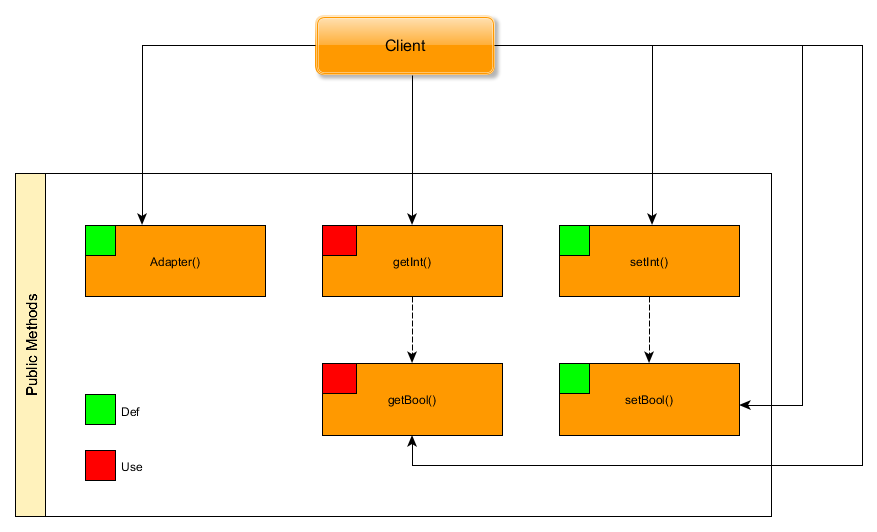
\includegraphics[width=0.3\textwidth]{./Adapter/Class/CallGraph.png}
	\caption{Data Flow Graph: \textit{bool\_value}}
	\label{CAdataflow}
\end{figure}


\subsubsection{Tests}
abbiamo fatto test sia di unit� che di interazione:

spara rassegna test $(i tipi elencati in idee_per_test)$

\section{Object Adapter}


\section{Proxy}

\section{Decorator}

\section{Composite}

-A � di tipo variabile/complessit� dovuta a topologia, rappresentato la nostra microarchitettura tramite  Data Flow graph/Class Dependency graph abbiamo deciso  di utilizzare il criterio di copertura all uses(rispetto a all defs)/all edges(rispetto a all nodes) 
-B � di tipo K,...
\section{Observer}

\section{State}

\section{Visitor}

\


\chapter{Conclusioni}

In questo elaborato abbiamo mostrato un sistema in grado di riconoscere automaticamente i muri di una planimetria, indipendentemente dalla notazione grafica utilizzata. In questo programma, se i muri rientrano nelle tipologie citate, � indipendente dagli altri standard e non necessita di informazioni aggiuntive per svolgere il proprio compito.
Dalla bont� dei risultati mostrati nel paragrafo precedente si pu� notare che quello presentato � un metodo valido per l'individuazione di muri in planimetrie. Le idee di base, in parte ispirate agli articoli \cite{1} e \cite{5} e in parte sviluppate ex novo, si sono dimostrate valide per raggiungere l'obiettivo prefissato. A sostegno di quanto appena detto viene ricordato quanto riportato nel capitolo precedente: ossia il fatto che i nostri risultati sono molto simili a quelli ottenuti da CVC ed in alcuni casi sono risultati anche migliori.
Con l'utilizzo di queste idee appena esposte sarebbe possibile arrivare ad un riconoscimento al 100\% indipendente dagli standard grafici utilizzati solo con un'aggiunta di codice che, riconosciuti i muri non pieni, si limiti a riempirli. Una volta raggiunto questo obiettivo un altro sviluppo futuro potrebbe essere il riconoscimento (gi� effettuato da CVC) di altri elementi strutturali quali porte, finestre e stanze.

\addcontentsline{toc}{chapter}{Bibliografia}
\begin{thebibliography}{99}

\bibitem{1} Lluis-Pere de las Heras, David Fernandez, Ernest Valveny, Josep Llados and Gemma Sanchez, ``Unsupervised Wall Detector in Architectural Floor Plans,'' in 12th International Conference on Document Analysis and Recognition, 2013.

\bibitem{2} P. Dosch, K. Tombre, C. Ah-Soon, and G. Masini, ``A complete system for the analysis of architectural drawings,'' International Journal on Document Analysis and Recognition, vol. 3, pp. 102 \verb0-0 116, 2000.

\bibitem{3} T. Lu, H. Yang, R. Yang, and S. Cai, ``Automatic analysis and integration of architectural drawings,'' International Journal on Document Analysis and Recognition, vol. 9, pp. 31 \verb0-0 47, 2007.

\bibitem{4} S. Mace, H. Locteau, E. Valveny, and S. Tabbone, ``A system to detect rooms in architectural floor plan images,'' in Proceedings of the 9th IAPR International Workshop on Document Analysis Systems, 2010, pp. 167\verb0-0 174.

\bibitem{5} Lluis-Pere de las Heras, David Fernandez, Ernest Valveny, Josep Llados and Gemma Sanchez, ``Statistical segmentation and structural recognition for floor plan interpretation,''  2013.

\bibitem{6} S. Ahmed, M. Liwicki, M. Weber, and A. Dengel, ``Improved automatic analysis of architectural floor plans,'' in Proceedings of the 11th International Conference on Document Analysis and Recognition, 2011.

\end{thebibliography}
\addcontentsline{toc}{chapter}{Elenco delle Figure}\listoffigures
\end{document}
